\section{PFunc: A Design Overview}
\label{sec:design}
 
Existing solutions for task parallelism do not offer users control over the
``little details''  that determine application performance; for example, 
Table~\ref{tbl:cilk_runtime} lists the execution details in Cilk, which 
cannot be tweaked by users.
%
\begin{table}
\centering
\begin{tabular}{|c|l|}
\hline
Detail & Explanation \\
\hline
Task priority & $\rightarrow{}$ No priorities. \\
\hline
Task scheduling policy & $\rightarrow{}$ Depth-first execution. \\
\hline
Task stealing policy & $\rightarrow{}$ Breadth-first theft. \\
\hline
Task affinity & $\rightarrow{}$ Executed by thread encountering the \textit{spawn}. \\
              & $\rightarrow{}$ Can be randomly stolen by \textit{any} thread. \\
\hline
Task graph structure & $\rightarrow{}$ Tree. \\
                     & $\rightarrow{}$ Imposed by the \textit{fork-join} model. \\
\hline
Task groups & $\rightarrow{}$ Tasks have no knowledge of one another. \\
            & $\rightarrow{}$ Entire task subtrees can be canceled. \\
\hline
\end{tabular}
\label{tbl:cilk_runtime}
\caption{Table listing the various ``little details'' in Cilk, which cannot be
tweaked by users either at compile-time or runtime.}
\end{table}
%
As a result, task parallelism only benefits a circumscribed set of
applications.
%
In order for task parallelism to be widely adopted, it is necessary to design
tools that have configurability and extensibility as their key features; 
PFunc, is designed to be such a tool.
%
PFunc uses the generic programming methodology to make it both configurable
and extensible without any runtime penalties; by default, PFunc can be used
\emph{as is} and does not require any configuration or extensions.
%
In this section, we explore the various components that constitute PFunc at
runtime as well as the functionality of these components.

\subsection{Software Architecture}
\label{subsec:software_architecture}

The primary goal of PFunc is to enable users to portably execute tasks
(asynchronous computations) on shared memory.
%
To achieve this goal, it interfaces with various low-level components and
user applications (see Figure~\ref{fig:software_architecture}).
%
PFunc uses user-level threads to execute tasks; therefore, it interfaces with
an underlying threading library (which is operating system specific). 
%
For example, on most UNIX-based operating systems, PFunc uses POSIX threads to
execute user tasks.
%
In PFunc, users are allowed to execute tasks on particular processors (i.e.,
set a task's affinity); this capability is necessary for optimal performance on
heterogeneous architectures.
%
In order to support setting task affinities, it is necessary to accurately map
individual threads to specific processors --- a capability that, currently,
only the operating systems provide; hence, PFunc interfaces with operating
systems.
%
PFunc implements and uses many concurrent data structures and algorithms. 
%
For maximum efficiency, these data structures and algorithms are implemented
using custom synchronization primitives that are built on top of
processor-specific atomic operations; hence, PFunc directly interfaces with the
hardware.
%
Finally, PFunc allows users to collect various hardware statistics about their
applications' execution  through the ``performance profiler'' component, which
in turn interfaces with the Performance Application Programming Interface
(PAPI; see Section~\ref{sec:perf}).

\begin{figure}
\centering
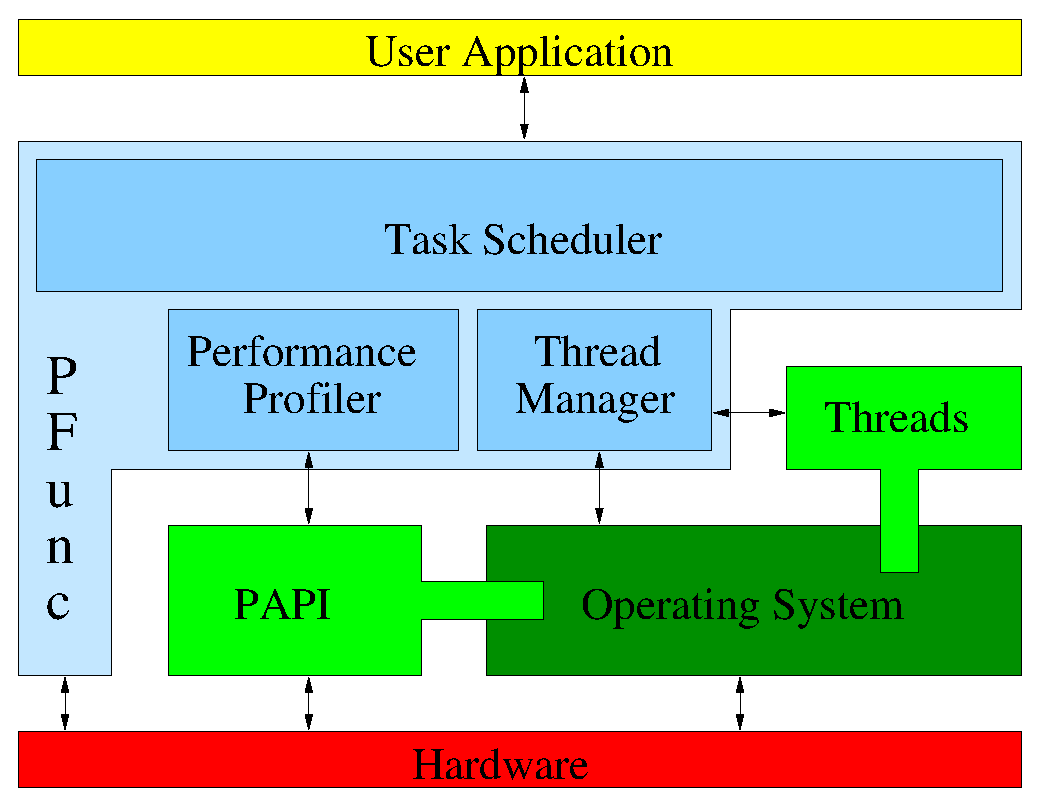
\includegraphics[width=.8\textwidth]{figs/architecture}
\caption{An overview of the software architecture of PFunc; only the relevant
components are shown. Components linked by arrows interface with each other.
Protrusion of one component into another implies that a part of the former
component is implemented in the latter (e.g., threads are partly implemented in
the operating system). Performance Application Profiling Interface (PAPI) is a
profiling library used for collecting hardware statistics.}
\label{fig:software_architecture}
\end{figure}

\subsection{Components of PFunc}
\label{subsec:pfunc_components}

The design of PFunc revolves around providing users control over six ``little
details'' related to task execution: priorities, scheduling, stealing,
affinities, graph structure, and groups.
%
As PFunc's design is ``lifted'' from the designs of existing task parallel
solutions, many components in PFunc correspond one-to-one with components in
other task parallel solutions with one important difference --- PFunc's
components can be configured and/or extended.
%
As shown in Figure~\ref{fig:runtime}, PFunc's components fit into three
categories: \textit{user-provided} (gold colored), \textit{generated} (pink
colored), and \textit{fixed} (blue colored).
%
User-provided components (work, task queue, and task predicates) are
implemented by the users to suit their needs.  
%
The task queue and the task predicate components from a logical grouping called
the task scheduler.
%
PFunc provides a number of built-in choices for the user-provided components;
hence, for many applications, PFunc works ``out-of-the-box''. 
%
However, if these built-in choices do not meet the users requirements, they may 
implement their own user-provided components.
%
Generated components (attribute, task, and task manager) are automatically
created at compile-time using information from the user-provided components.
%
The user-provided and generated components can be configured and/or extended to
create a variety of configurations of PFunc (see Section~\ref{sec:custom}).
%
Fixed components are non-configurable and include group, thread manager,
exception handler, and performance profiler.
%
In practice, PFunc components are implemented as \Cpp{} classes; hence, PFunc
at runtime consists of one or more objects of these classes that are
interacting with each other.
%

\begin{figure}
\centering
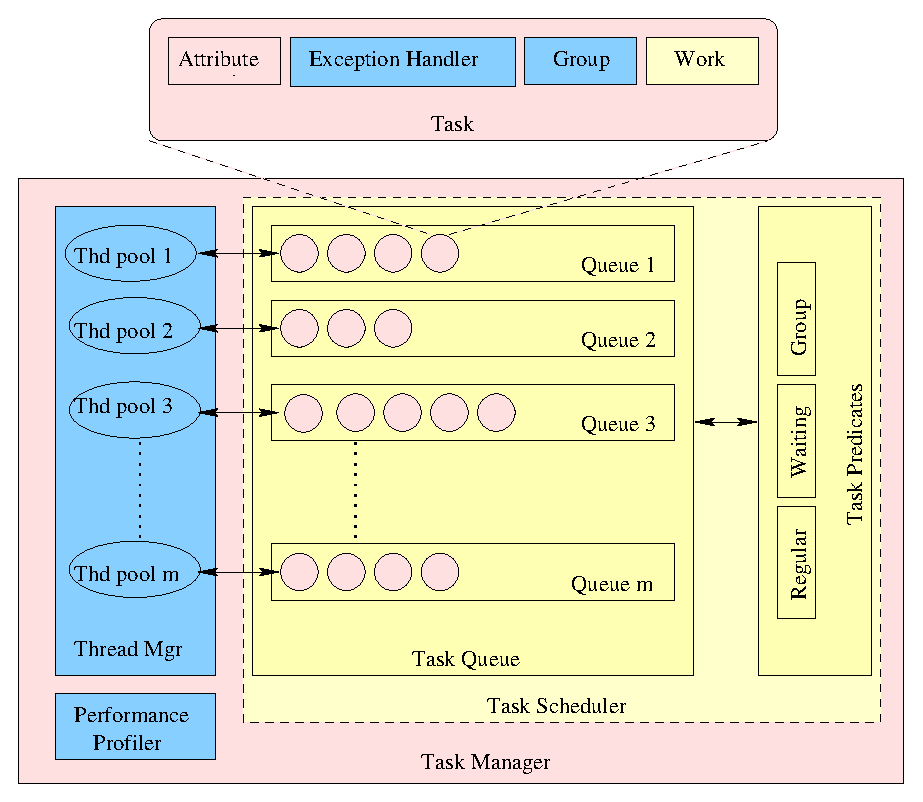
\includegraphics[width=0.8\textwidth]{figs/runtime}
\caption{An overview of the different components in PFunc at runtime.
Components colored yellow (task queue, task predicate, and work) are
user-provided. Components colored pink (attribute, task, and task manager) are
generated. Components colored blue are fixed. PFunc allows users to customize
both the user-provided and generated components.}
\label{fig:runtime}
\end{figure}

\subsection{User-provided Components}
\label{subsec:user_provided}

\subsubsection{Task Scheduler}
%
This component is a logical grouping of the task queue and the task predicate
components.
%
The task scheduler is primarily responsible for choosing the next task to be
executed by each thread. 
%
The task queue and the task predicate components are chosen at compile-time
based on the task scheduling policy selected by the user (see
Section~\ref{sec:custom}).
%
Users can choose from one of the four built-in scheduling policies
(\code{cilkS}, \code{prioS}, \code{lifoS}, and \code{fifoS}) or choose to 
implement their own scheduling policy.
%
For the built-in scheduling policies, the task queue and task predicate
components are pre-defined.
%
However, if users choose to implement their own scheduling policy, they must 
define the task queue and the task predicate components.
%
 
There are two situations in which the task scheduler is used: when a task
is spawned and inserted into a task queue, and when a thread is ready to
execute a task and this task must be selected from the task queue.
%
There are three scenarios in which a thread is ready to execute a task. 
%
In the first scenario, the thread is idle and is looking for a task to execute; 
this is called a \emph{regular} scheduling point.
%
In the second scenario, the thread suspends the parent task it is executing
because the parent task starts waiting on one or more of its children to
complete execution.  
%
Therefore, a new task must be chosen for this thread to execute; this is called
a \emph{waiting} scheduling point.
%
In the third scenario, the thread suspends execution of a task because the task
has entered a wait for a group barrier operation; this is called a \emph{group}
scheduling point.
%

\paragraph{Task Queue}
%
The task queue manages multiple internal queues that store references to
spawned tasks, and supports two atomic operations: \func{put} and \func{get}.
%
The \func{put} function is used to add a newly spawned task to a user-specified
queue.
%
The \func{get} function is used to retrieve a task from the task queue. 
%
The exact queue from which \func{get} retrieves the task is determined jointly
with the task predicate component. 
%
The nature of the internal queues used by the task queue component reflects the
scheduling policy being implemented.
%
For example, for the \code{cilkS} scheduling policy, \code{std::deque} is used
as the type of each internal queue.
%
Similarly, for the \code{lifoS} scheduling policy, \code{std::stack} is used
as the type of each internal queue.

\paragraph{Task Predicate}
%
This component is composed of three predicate pairs --- one pair of predicates
for each scheduling point. 
%
The \code{regular\_predicate\_pair} is used during the regular scheduling
point, \code{waiting\_predicate\_pair} during the waiting scheduling point, and
\code{group\_predicate\_pair} during the group scheduling point.
%
The first predicate of each pair is used to enforce scheduling when the calling
thread's \emph{own} queue is non-empty; the second predicate of each pair is
used when the calling thread's own queue is empty and a task must be
\emph{stolen} from another queue.
 
%
In conjunction with the task queue, the task predicate helps implement a
variety of scheduling policies.
%
The task predicate is used when a new task has be chosen for execution --- when
any of the three scheduling points  is reached.
%
When a thread needs a task to execute, it (via the task manager) calls the
\func{get} function of the task queue; the predicate pair corresponding to the
scheduling point is determined and passed in as an argument to \func{get}.
%
Then, \func{get} checks if the calling thread's own queue is non-empty. 
%
If it is non-empty, depending on the scheduling policy, candidate tasks are 
selected and the \emph{own} predicate is applied to those tasks.
%
The first candidate task from the calling thread's own queue to satisfy the 
predicate is returned to the calling thread for execution.
%
If the calling thread's own queue is empty or if there are no eligible tasks in
it, \func{get} tries to steal a task from another randomly selected queue, at
which point, the \emph{steal} predicate is used.

\begin{figure}
\centering
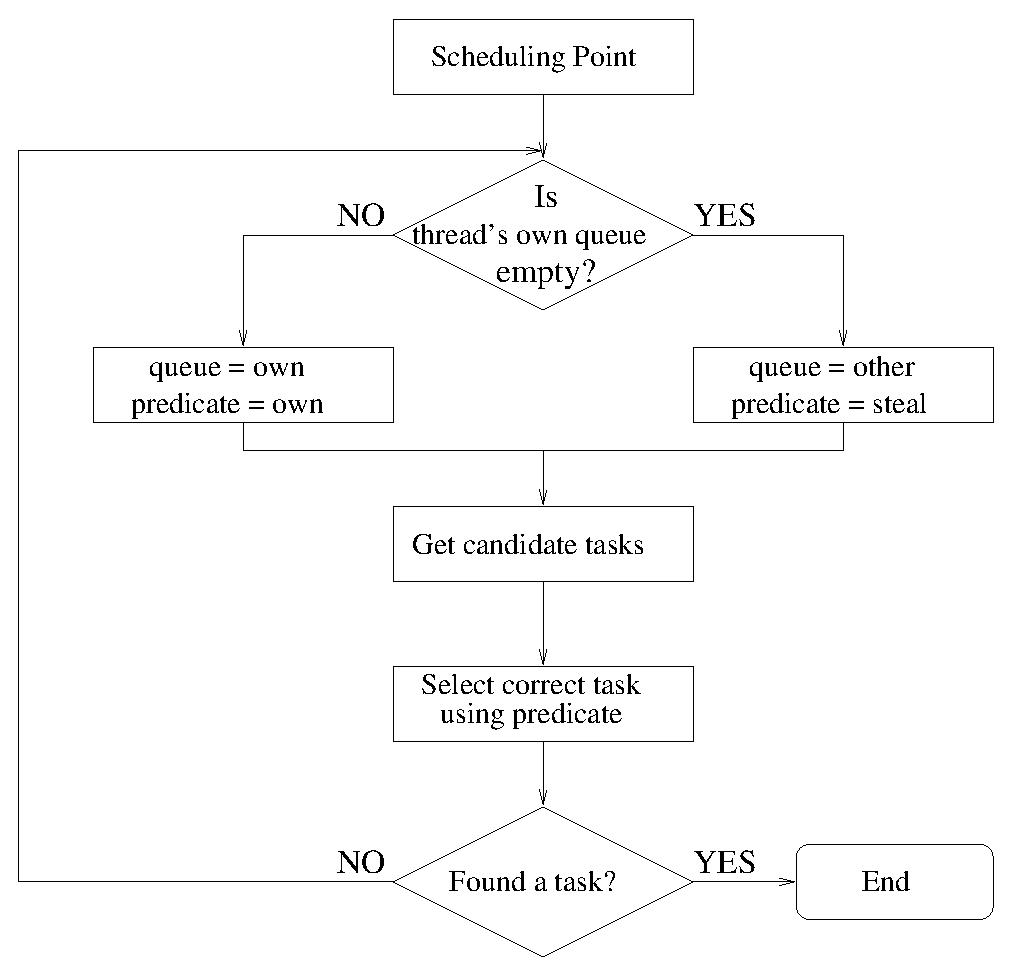
\includegraphics[width=0.7\textwidth]{figs/scheduling}
\caption{Flowchart depicting the task selection process at a scheduling point.}
\label{fig:scheduling}
\end{figure}

\paragraph{Work}
%
The main purpose of PFunc is to enable asynchronous execution of computations.
%
Work is the generic representation of a computation and is a part of the task.
%
In PFunc, computations are restricted to be functions or function objects that 
meet certain constraints.

\subsection{Generated Components}
\label{sec:auto_generated}

\subsubsection{Attribute}
\label{subsubsec:attribute}
%
The attribute component is central in providing users control over ``little
details'' such as scheduling, priority, affinity, task graph structure, and
grouping.
%
Each task contains an attribute, which in turn is made up of six
sub-attributes: \emph{priority}, \emph{queue\_number}, \emph{num\_waiters},
\emph{grouped}, \emph{level}, and \emph{nested}.
%
As there is a task associated with each asynchronous computation, there is also
an attribute associated with each asynchronous computation.
%
To control the execution of a task, users can specify the value for the
required sub-attributes of the task's attribute at the time of spawning.
%
The role of each of these six sub-attributes is summarized below.

\paragraph{priority} Many task scheduling policies require that tasks 
themselves provide hints to help scheduling.
%
For example, the built-in \code{prioS} scheduling policy requires each task to
have a priority.
%
The priority sub-attribute can be used to provide hints to the scheduler
component to help realize customized scheduling policies.
 
\paragraph{queue\_number} PFunc allows control over the affinity of a task
by allowing users to specify the task queue (numbered $[0..n)$, where $n$ is 
the total number of queues) on which the task must be spawned.
%
This is a departure from the methodology of existing solutions for task
parallelism, where a task is always put on the queue serviced by the spawning
thread. 
%
In PFunc, the task is put on the queue serviced by the spawning thread only
if a queue number is not specified while spawning the task.
 
\paragraph{num\_waiters} In PFunc, a task can have multiple parents, which 
results in the task graph structure being a DAG, not just a tree.
%
To support DAG-shaped task graph structures, it is necessary to be able to 
deliver status notifications regarding a task to all its parents.
%
The value of the num\_waiters sub-attribute gives the number of parents for the
task.
%
If this sub-attribute is unspecified for a task, that particular task is
assumed to have a single parent.
 
\paragraph{grouped} PFunc supports SPMD-style parallelization through task
groups.
%
When a task is part of a group, it is automatically given a \emph{rank} in the 
group, which it can use to communicate with the members of its own group.
%
However, when a task is attached to a group, extra instructions are added to 
the critical path (see Section~\ref{subsubsec:group}); therefore, tasks that
use PFunc's group infrastructure incur a performance penalty.
%
To avoid performance loss incurred from a task's membership in a group, the
grouped sub-attribute can be modified so that PFunc only associates the task
with its group when necessary.
%
Most task parallel programs do not make use of groups; by default, tasks are
not attached to \textit{any} group (i.e., grouped sub-attribute is unset)

\paragraph{level} This sub-attribute is used by the task scheduler to
ensure that the thread does not exhaust its stack space by stealing
incorrectly.
%
An important function of the task scheduler component is to ensure that the
underlying system resources are not exhausted. 
%
Thread stack space is one such resource.
%
In PFunc, three of the built-in scheduling policies (\code{cilkS},
\code{lifoS}, and \code{fifoS}) utilize the level sub-attribute to accurately
determine the depth of a task in the task graph.
%
Then, by enforcing a stealing predicate that prohibits a thread from stealing
tasks that are higher (closer to the root) in the task graph than the task 
currently suspended by the thread, thread stack space is conserved.
%

\paragraph{nested} PFunc inherently supports nested parallelism, in which
a task is allowed to spawn other tasks recursively.
%
As there may be more tasks than threads, to support nested parallelism we
need to suspend a parent task to execute a child task.
%
Such task suspension is automatically carried out at both the waiting and 
group scheduling points.
%
However, PFunc's nested sub-attribute allows users to prevent automatic task
suspension at these synchronization points by turning off nested parallelism at
the task level.
%

\subsubsection{Task}
\label{subsubsec:task}
%
The task is PFunc's representation of an asynchronous computation; it contains
the attribute, group, exception handler, and work that is related to the
computation's execution.
%
There is one ``active'' task for each spawned computation.
%
Task interfaces with users on one end and the task scheduler and task manager
on the other end.
%
When a spawned computation completes its execution, the task delivers its
completion notifications to all its parent tasks.
%
The number of completion notifications delivered depends on that particular
task's num\_parents sub-attribute.
%
After all the completion notifications have been delivered, the task is 
terminated; at this point, the task is ``inactive'' and can be used to spawn 
another asynchronous computation.
%
When a task enters either a waiting or group scheduling point, if the task is 
nested, the task triggers the task manager; the task manager in turn starts a
scheduling cycle.
%

\subsubsection{Task Manager}
\label{subsubsec:task_manager}

The task manager is PFunc's runtime; it is the component that glues together
the task, task scheduler, thread manager, and performance profiler components.
%
The task manager's responsibilities can be fit into three categories:
initialization, scheduling, and shut down.
 
\paragraph{Initialization:} During initialization, users provide two pieces of
information: the number of task queues and the number of threads per task
queue.
%
The task manager uses this information to create the specified number of task 
queues and attaches the requested number of threads to each queue. 
%
With this facility, users can create an $m\times{}n$ mapping between queues and
threads.
%
When $m=n$, there is one thread attached to each queue; this is called the 
\emph{work-stealing} configuration.
%
When $m=1$, there is one queue to which all $n$ threads are attached; this is
called the \emph{work-sharing} configuration.
%
Optionally, users can also specify both the affinity of each thread to
individual processors, and the hardware statistics to be collected (see
Section~\ref{sec:perf}).
%
At the end of initialization, the task scheduler, the thread manager, and
the performance profiler are configured, and the task manager is ready to be
used to spawn and execute tasks asynchronously.

\paragraph{Scheduling:} This phase can alternately be called the
\emph{spawn-execute-sync} phase. 
%
When a task is spawned, the task manager is responsible for placing it in the
appropriate queue.
%
When a thread reaches a tasks scheduling point, the thread manager interfaces
with the task scheduler to retrieve an eligible task for this thread to
execute.
%

\paragraph{Shut down:} When the library runtime is no longer needed,
the task manager is responsible for the cleanup of system resources.

\subsection{Fixed Components}
\label{subsec:fixed}

\subsubsection{Group}
\label{subsubsec:group}
%
It is difficult to express all segments of a program in the task parallel
model, therefore, PFunc allows users to mix task parallelism with SPMD-style
programming.
%
The group component is central in providing the support required for SPMD-style
programming. 
%
A task is allowed to be a member of only one group, and group membership is
assigned to a task at the time of spawning.
%
Tasks within the same group can communicate using built-in synchronization
operations. 
%
Each group has the following three pieces of information associated with it:

% Id
\paragraph{Id} This is an integer that uniquely identifies each group and
may be used for debugging purposes.
% Size
\paragraph{Size} Also an integer, this specifies the maximum number of
tasks allowed in the group.
%
The group component can be enabled or disabled for each individual task at
spawn time using the grouped sub-attribute (see
Section~\ref{subsubsec:attribute}).
%
When a task is spawned with its grouped sub-attribute enabled, that task is
given a unique rank in the group at the time of spawning.
%
The rank of a task is an integer in the range $[0..Size)$, and is valid only
when the task is ``active''.
% Barrier
\paragraph{Barrier type} PFunc provides three types of barriers:
\emph{spinning}, \emph{waiting}, and \emph{stealing}. 
%
The value of the barrier type determines which of the three barriers is in use.
%
Spinning barriers are the default.
%
Threads executing tasks in a spinning barrier are incapable of executing other
tasks while these tasks wait on the barrier because the threads must actively
poll for barrier completion.
%
Consequently, the spinning barrier is most useful when all the tasks involved
in the barrier are tightly coupled.
%
Furthermore, for the spinning barrier to work properly, there must be a 
separate thread for each task executing the barrier.
% 
In other words, the size of the group must be less than or equal to the number
of threads used to execute the library instance, or a deadlock may occur.
%
Waiting barriers are useful when system resources need to be conserved. 
%
In waiting barriers, the thread executing a blocked task is suspended from
execution until the barrier is completed.
%
Like the spinning barrier, the waiting barrier also requires that the size of
the group be less than or equal to the number of threads in the system.
%
Finally, stealing barriers offer the speed of spinning barriers and the
efficiency of waiting barriers.
%
When a task is waiting at a stealing barrier, the thread that is executing the
task can suspend the task and execute another eligible task.
%
Therefore, if the tasks involved in a barrier are not tightly coupled, the 
threads executing these tasks can do useful work.
%
The stealing barrier also requires that the number of tasks in the group be
less than or equal to the number of threads.
%
This constraint is a result of the lack of support for true task suspension in
PFunc.\footnote{True task suspension requires that the entire task (with its
stack) be suspended and later resumed by any other thread}. 
%

\subsubsection{Thread Manager}
\label{subsubsec:thread_manager}
%
As PFunc operates exclusively in shared memory, it makes uses of system threads
to execute its tasks.
%
This component is an abstraction that provides portable means of launching,
killing, and yielding threads on various platforms.
%
When PFunc is initialized, the thread manager launches as many threads as
requested and makes them available to service specific task queues.
%
Also, when the underlying system allows for it, the thread manager provides a
portable means of setting each thread's processor affinities --- an important
requirement for optimal performance of many applications.
%
This feature can be used in conjunction with the task attribute to control the
physical processors on which individual tasks are executed.
%
For example, during library initialization, users can tie individual threads 
down to particular processors and determine the task queues serviced by these
threads.
%
Then, using the affinity sub-attribute, tasks can be spawned on particular queues.

\subsubsection{Exception Handler}
\label{subsubsec:exception_handler}

The exception handler aids users in the development of robust applications by
ensuring sensible handling of exceptions in a parallel environment.
%
A parallel execution environment presents two challenges with respect to
exception handling. 
%
First, many PFunc routines are inserted between the child (callee) task which
is throwing the exception and the parent (caller) task that is catching it. 
%
Furthermore, the child and the parent tasks may be executed by different
threads. 
%
Therefore, exceptions need to be transported across many functions and/or
threads.
%
Second, unlike in a sequential environment, the parent task's execution is not always 
suspended until its child task returns. 
%
Therefore, an exception thrown by a task must be stored safely until its parent
task is ready to handle the exception (i.e., waits for the completion of the
throwing task).
%
PFunc's exception handler not only tackles both these challenges, but is also 
capable of delivering exception objects to multiple parent tasks.
%
Therefore, users can handle exceptions as if they were running a sequential
program. 
%
                                
The exception handler defines a new exception class, \code{pfunc::exception},
which extends \code{std::exception} to provide two additional pieces of
information to the users. 
%
First, the trace of the tasks and/or functions through which an exception
object was transported is exposed to the users.
%
Second, if a task terminated as a result of a failed system call or an error
internal to PFunc, this error code is provided to the users.
%
When a task throws an exception, the task is terminated (deactivated) and the
thrown exception is cloned and stored within the task (which is inactive).
%
Cloning is necessary in order to transport the exceptions across multiple tasks
and/or functions without loss of information.
%
Cloning requires that the exceptions objects inherit from either
\code{pfunc::exception} or \code{std::exception}; exception objects that do not
meet this requirement are discarded and a \code{pfunc::exception} with an
``unknown error'' description is propagated in their place.
%
As exception objects may need to be transported from a deeply-nested task to a
top-level task, \code{pfunc::exception} also allows users to add tracing
information that can be used to like a pseudo stack trace.
%
After additional tracing information has been added, the exception object can
be re-thrown to the next higher-level task.
% 

Unfortunately, the exception handler has two shortcomings. 
%
First, when a parent task waits on its children to complete, the exception 
handler must actively check for exceptions.
%
This adds an extra branch in the critical path and results in a small
performance penalty.
%
To remedy this, the exception handler component is disabled by default, and 
can be enabled using a compile-time flag.
%
Second, when a task throws an exception, all the tasks spawned by the throwing
task may have to be cancelled --- a capability that is currently
lacking in the exception handler.

\subsubsection{Performance Profiler}
\label{subsubsec:performance_profiler}

Achieving optimal parallel performance often requires tuning various parameters
such as task scheduling policy, task affinities, etc.
%
To help with such tuning, PFunc provides a performance profiler component that
allows users to collect various hardware statistics related to their
application run.
%
To collect the hardware statistics, this component interfaces with the
Performance Application Programming Interface (PAPI), a production-grade,
open-source, and portable low-level interface.
%
The performance profiler component allows users to specify particular events
(both PAPI presets and native) that they wish to monitor at the time of library
initialization.
%
Then, using PAPI, the performance profiler collects the required hardware 
statistics that can be retrieved at the end of the application run.
%
Shortly, the performance profiler will also be able to collect various
statistics about PFunc's components (e.g., number of steals per thread and load
per thread) that occurred during an application run.
%
